%% start of file `template.tex'.
%% Copyright 2006-2015 Xavier Danaux (xdanaux@gmail.com).
%
% This work may be distributed and/or modified under the
% conditions of the LaTeX Project Public License version 1.3c,
% available at http://www.latex-project.org/lppl/.


\documentclass[11pt,a4paper,sans]{moderncv}        % possible options include font size ('10pt', '11pt' and '12pt'), paper size ('a4paper', 'letterpaper', 'a5paper', 'legalpaper', 'executivepaper' and 'landscape') and font family ('sans' and 'roman')
\usepackage{ragged2e}
\usepackage{lastpage}
\usepackage[official]{eurosym}
\usepackage{fancyhdr}
\usepackage{pdfpages}
%\fancyfoot[C]{ \thepage\ / \pageref{LastPage}}
\fancyfoot[C]{ \thepage\ / 5}
% moderncv themes
\moderncvstyle{classic}                             % style options are 'casual' (default), 'classic', 'banking', 'oldstyle' and 'fancy'
\moderncvcolor{blue}                               % color options 'black', 'blue' (default), 'burgundy', 'green', 'grey', 'orange', 'purple' and 'red'
%\renewcommand{\familydefault}{\sfdefault}         % to set the default font; use '\sfdefault' for the default sans serif font, '\rmdefault' for the default roman one, or any tex font name
%\nopagenumbers{}                                  % uncomment to suppress automatic page numbering for CVs longer than one page

% character encoding
%\usepackage[utf8]{inputenc}                       % if you are not using xelatex ou lualatex, replace by the encoding you are using
%\usepackage{CJKutf8}                              % if you need to use CJK to typeset your resume in Chinese, Japanese or Korean
\renewcommand*{\namefont}{\fontsize{20}{40}\mdseries\upshape}

% adjust the page margins
\usepackage[scale=0.75]{geometry}
%\setlength{\hintscolumnwidth}{3cm}                % if you want to change the width of the column with the dates
%\setlength{\makecvtitlenamewidth}{10cm}           % for the 'classic' style, if you want to force the width allocated to your name and avoid line breaks. be careful though, the length is normally calculated to avoid any overlap with your personal info; use this at your own typographical risks...

% personal data
\name{Fabian}{Gruber}
%\title{Resumé title}                               % optional, remove / comment the line if not wanted
\address{Anna-Stainer-Knittel-Weg 3/5/4}{6020 Innsbruck, \"Osterreich}% optional, remove / comment the line if not wanted; the "postcode city" and "country" arguments can be omitted or provided empty
\phone[mobile]{+43~650~2587521}                   % optional, remove / comment the line if not wanted; the optional "type" of the phone can be "mobile" (default), "fixed" or "fax"
%\phone[fixed]{+2~(345)~678~901}
%\phone[fax]{+3~(456)~789~012}
\email{Fabian.Gruber@uibk.ac.at}                               % optional, remove / comment the line if not wanted
%\homepage{www.johndoe.com}                         % optional, remove / comment the line if not wanted
%\social[linkedin]{john.doe}                        % optional, remove / comment the line if not wanted
%\social[twitter]{jdoe}                             % optional, remove / comment the line if not wanted
%\social[github]{jdoe}                              % optional, remove / comment the line if not wanted
%\extrainfo{additional information}                 % optional, remove / comment the line if not wanted
\photo[64pt][0.4pt]{fabian_bewerbungsfoto}                       % optional, remove / comment the line if not wanted; '64pt' is the height the picture must be resized to, 0.4pt is the thickness of the frame around it (put it to 0pt for no frame) and 'picture' is the name of the picture file
%\quote{}                                 % optional, remove / comment the line if not wanted

% bibliography adjustements (only useful if you make citations in your resume, or print a list of publications using BibTeX)
%   to show numerical labels in the bibliography (default is to show no labels)
\makeatletter\renewcommand*{\bibliographyitemlabel}{\@biblabel{\arabic{enumiv}}}\makeatother
%   to redefine the bibliography heading string ("Publications")
%\renewcommand{\refname}{Articles}

% bibliography with mutiple entries
%\usepackage{multibib}
%\newcites{book,misc}{{Books},{Others}}
%----------------------------------------------------------------------------------
%            content
%----------------------------------------------------------------------------------
\begin{document}
%\begin{CJK*}{UTF8}{gbsn}                          % to typeset your resume in Chinese using CJK

%-----       letter       ---------------------------------------------------------
% recipient data
\recipient{Airborne Technologies GmbH \\z.H. Teresa Mancevski}{Viktor Lang Stra{\ss}e 8\\A-2700 Wiener Neustadt}
\date{18. Dezember 2017}
\opening{\textbf{Betreff: Bewerbung als Mitarbeiter in der Datenverarbeitung} \\[0.5cm]   Sehr geehrte Frau Mancevski!}

\closing{Mit besten Gr\"{u}{\ss}en,}
\enclosure[Anhang]{Lebenslauf, Publikationsliste, Diplombescheid und Zeugnis der zweiten Diplompr\"ufung}        % use an optional argument to use a string other than "Enclosure", or redefine \enclname

\makelettertitle
\justify
Erfahrungen im Bereich der Geoinformation sammle ich bereits seit meinem Studium der Kulturtechnik und Wasserwirtschaft an der Universit\"at f\"ur Bodenkultur in Wien. Dort absolvierte ich neben den Grundlagenf\"achern auch den Wahlfachblock \emph{Vermessung, Fernerkundung und Geoinformation} und w\"ahlte das Fach Geodatenmanagement als Zweitfach der Diplompr\"ufung. Als Projektmitarbeiter an der Boku war ich in der Digitalisierung von Naturgefahrenereignissen und Gletschern anhand von Satellitendaten t\"atig. Auch in Innsbruck  besch\"aftige ich mit Arbeitsergebnissen der Fernerkundung, vor allem digitalen Gel\"andemodellen.

Aufgrund meiner langj\"{a}hrigen T\"atigkeit als Projektmitarbeiter an verschiedenen Universit\"{a}ten bringe ich Erfahrung beim selbstst\"{a}ndigen Arbeiten mit. Ich bin es gewohnt mich rasch in neue Themen einzuarbeiten und interessiere mich sehr f\"ur Fernerkundungsmethoden und deren Anwendung in verschiedensten Bereichen. So absolvierte ich vor kurzem den Onlinekurs der European Space Agency \emph{Introduction to radar remote sensing}.

Die auf der Homepage angef\"{u}hrten vergangenen Projekte Ihrer Firma haben mein Interesse geweckt. Homeoffice sowie ein Wochenstundenausma{\ss} von etwa 25 Stunden w\"urde mir erm\"oglichen weiter an meiner Dissertation und deren Abschluss zu arbeiten. Meine Gehaltsvorstellungen liegen bei 2508 \euro{} brutto  bei Vollzeitanstellung. Fr\"uhester Eintrittstermin w\"are der 12. Februar 2018.

\"{U}ber eine Einladung zu einem Gespr\"ach w\"urde ich mich freuen.

\makeletterclosing
\clearpage
%-----       resume       ---------------------------------------------------------
\makecvtitle


\section{Berufserfahrung}
\cventry{2013--heute   }{Wissenschaftlicher Mitarbeiter}{Institut f\"{u}r Geographie, Universit\"{a}t Innsbruck}{Innsbruck}{}{Forschungsprojekte: 
\begin{itemize}%
\item \emph{Shallow erosion dynamics in mountain grasslands of South Tyrol: Monitoring, process analysis and mitigation measures (EroDyn)}
  \begin{itemize}%
  \item Geodatenmanagement 
   \item Gel\"{a}ndeklassifizierung f\"{u}r automatisierte Blaikenkartierung
   \item Dispositionskartierung auf Landesebene
   \end{itemize}
\item \emph{ReBo -- Reliefklassifizierung aus ALS Daten als Grundlage f\"ur die Regionalisierung von Bodendaten}
  \begin{itemize}%
  \item Ableitung von Landschaftseinheiten mit maschinellem Lernen und automatisierten Gel\"{a}ndeklassifikationsalgorithmen 
  \item \emph{Gruber, F.E., Baruck, J., Geitner, C., 2017:  Algorithms vs. surveyors: a comparison of automated landform delineations and surveyed topographic positions from soil mapping in an Alpine environment. Geoderma 308, 9-25.}
  \item Bodenkundliche Feldarbeit
  \item Mitarbeit bei der Entwicklung der Java-Applikation \emph{SEPP} (Soil Evaluation in Planning Procedures) f\"{u}r Bodenfunktionsbewertungen
  \end{itemize}
\end{itemize}}
\cventry{2016--2017}{Lektor}{Institut f\"{u}r Geographie, Universit\"{a}t Innsbruck}{Innsbruck}{}{\"{U}bungen zur Statistik mit R (2 Semester)}
\cventry{2016--2017}{Bildungskarenz}{}{Innsbruck}{}{Arbeit an der Dissertation mit dem Arbeitstitel \emph{Digital terrain analysis to support field soil survey}}
\cventry{2011--2013}{Wissenschaftlicher Mitarbeiter}{Institut f\"{u}r Angewandte Geologie, BOKU}{Wien}{}{Forschungsprojekte: 
\begin{itemize}%
\item \emph{Hazard assessment for an expected dam break flood in the Hunza Valley, Pakistan: A combination of GIS, Remote Sensing, and computer simulation techniques}
\begin{itemize}%
  \item Dammbruch-Modellierung mit BREACH
  \item Hydraulische Modellierung mit FLO-2D
  \end{itemize}
\item \emph{Poverty Alleviation through Mitigation of Integrated High-Mountain Risk (PAMIR)}
\begin{itemize}%
  \item Kartierung von Naturgefahren, Gletschern und Infrastruktur mit GIS und Fernerkundungsmethoden
  \item \emph{Gruber, F.E., Mergili, M., 2013: Regional-scale analysis of high-mountain multi-hazard and risk indicators in the Pamir (Tajikistan) with GRASS GIS. Natural Hazards and Earth System Sciences 13: 2779-2796.}
  \end{itemize}
  \end{itemize}}
\cventry{2009--2010}{Projektmitarbeiter}{Institut f\"{u}r Angewandte Geologie, BOKU}{Wien}{}{Forschungsprojekt: 
\begin{itemize}%
\item \emph{Remote Geohazards Assessment in Tajikistan (TajHaz)}
\begin{itemize}%
  \item Kartierung von Naturgefahren und Gletscherseen anhand von Satellitenbildern  und GIS
  \item Feldarbeit in Tajikistan
  \end{itemize}
  \end{itemize}}

\cventry{2010--2011}{Tutor}{ Institut f\"ur Landschaftsentwicklung, Erholungs- und Naturschutzplanung, BOKU}{Wien}{}{Tutor f\"ur ArcGIS im Rahmen der LV \emph{Einf\"uhrung in GIS}}

\section{Ausbildung}
\cvitem{2002--2011}{Diplomstudium der Kulturtechnik und Wasserwirtschaft an der Universit\"{a}t f\"{u}r Bodenkultur (BOKU), Wien}
\cvitem{1993--2001}{Linz International School Auhof, Linz:
Abschluss mit Matura und International Baccalaureate (IB)}
\cvitem{1991--1993}{Volksschule Linz-Pichling}
\cvitem{1989--1991}{Lincoln Elementary School Pittsburgh, PA, USA}

\section{Diplomarbeit}
\cvitem{Titel}{\emph{The 2010 Attabad Landslide Dam Lake:
modeling and prediction of Lake Outburst
Floods}}
\cvitem{Betreuer}{Jean F. Schneider und Martin Mergili}

\section{Sprachen}
\cvitemwithcomment{Deutsch}{Muttersprache}{ }
\cvitemwithcomment{Englisch}{Verhandlungssicher}{ }
\cvitemwithcomment{Spanisch}{Grundkenntnisse}{ }
\cvitemwithcomment{Franz\"osisch}{Grundkenntnisse}{ }

\section{EDV-Kenntnisse}
\cvdoubleitem{Operating systems}{Linux (Ubuntu), Windows} {Languages}{R, Python, Bash}
\cvdoubleitem{Geographic information systems}{ArcGIS, GRASS, SAGA, QGIS } {Text- verarbeitung } {MS Word, Libreoffice,  \LaTeX{} with Texmaker}
\cvdoubleitem{Bild- verarbeitung}{GIMP, Inkscape} {Modellierungs- software } {FLO-2D, Ramms, Dan-3D}
\section{Hobbies}
\cvitem{G\"artnerei}{Mitarbeit beim Gemeinschaftsgarten der Vinzigemeinschaft Waldhuttl, Innsbruck}
\cvitem{Reisen}{Reisen durch Mittel- und S\"udamerika, Zentralasien, S\"udostasien und Madagaskar}


\clearpage

% Publications from a BibTeX file without multibib
%  for numerical labels: \renewcommand{\bibliographyitemlabel}{\@biblabel{\arabic{enumiv}}}% CONSIDER MERGING WITH PREAMBLE PART
%  to redefine the heading string ("Publications"): 
\renewcommand{\refname}{Publikationen}
\nocite{*}
\bibliographystyle{plain}
\bibliography{publications3}   
%\clearpage\end{CJK*}                              % if you are typesetting your resume in Chinese using CJK; the \clearpage is required for fancyhdr to work correctly with CJK, though it kills the page numbering by making \lastpage undefined
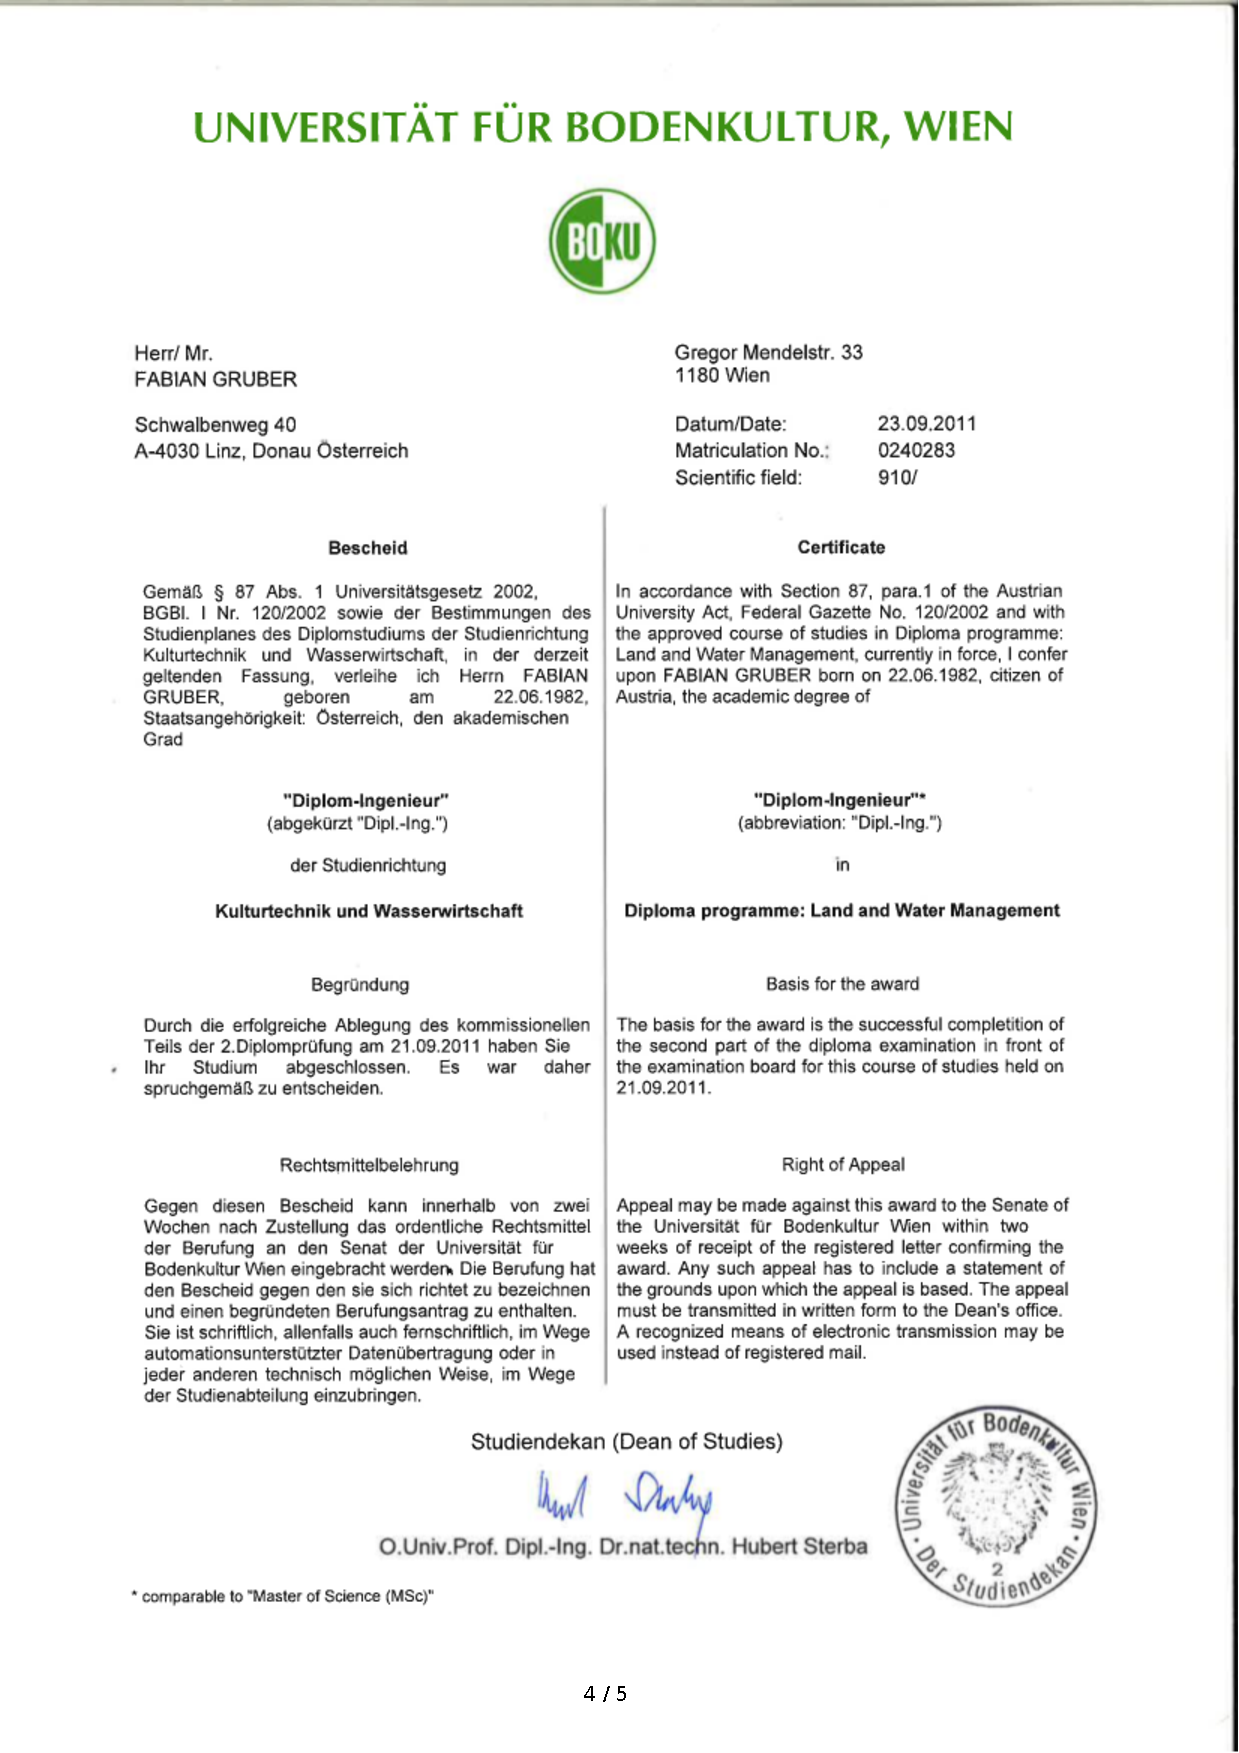
\includepdf{DP_seite4von5.pdf}
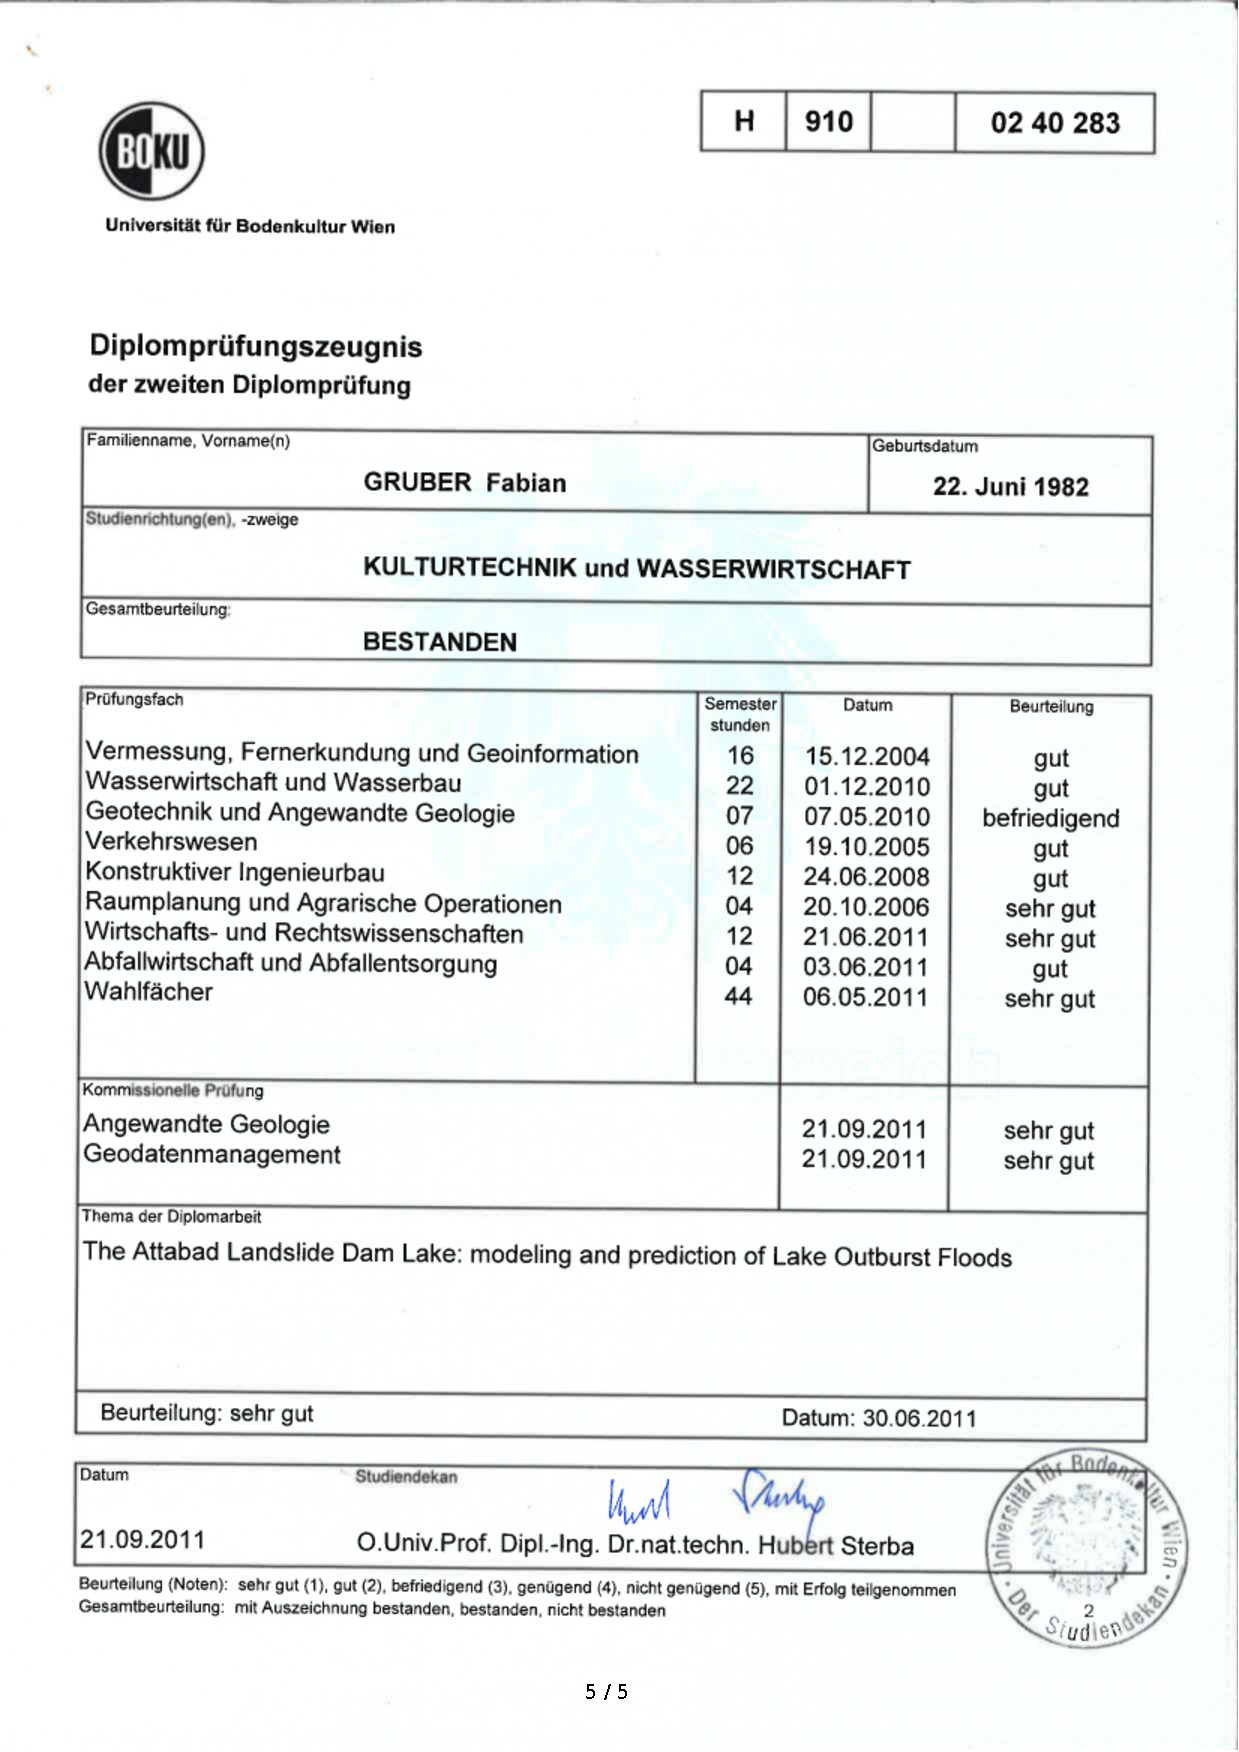
\includepdf{DP1_5von5.pdf}
%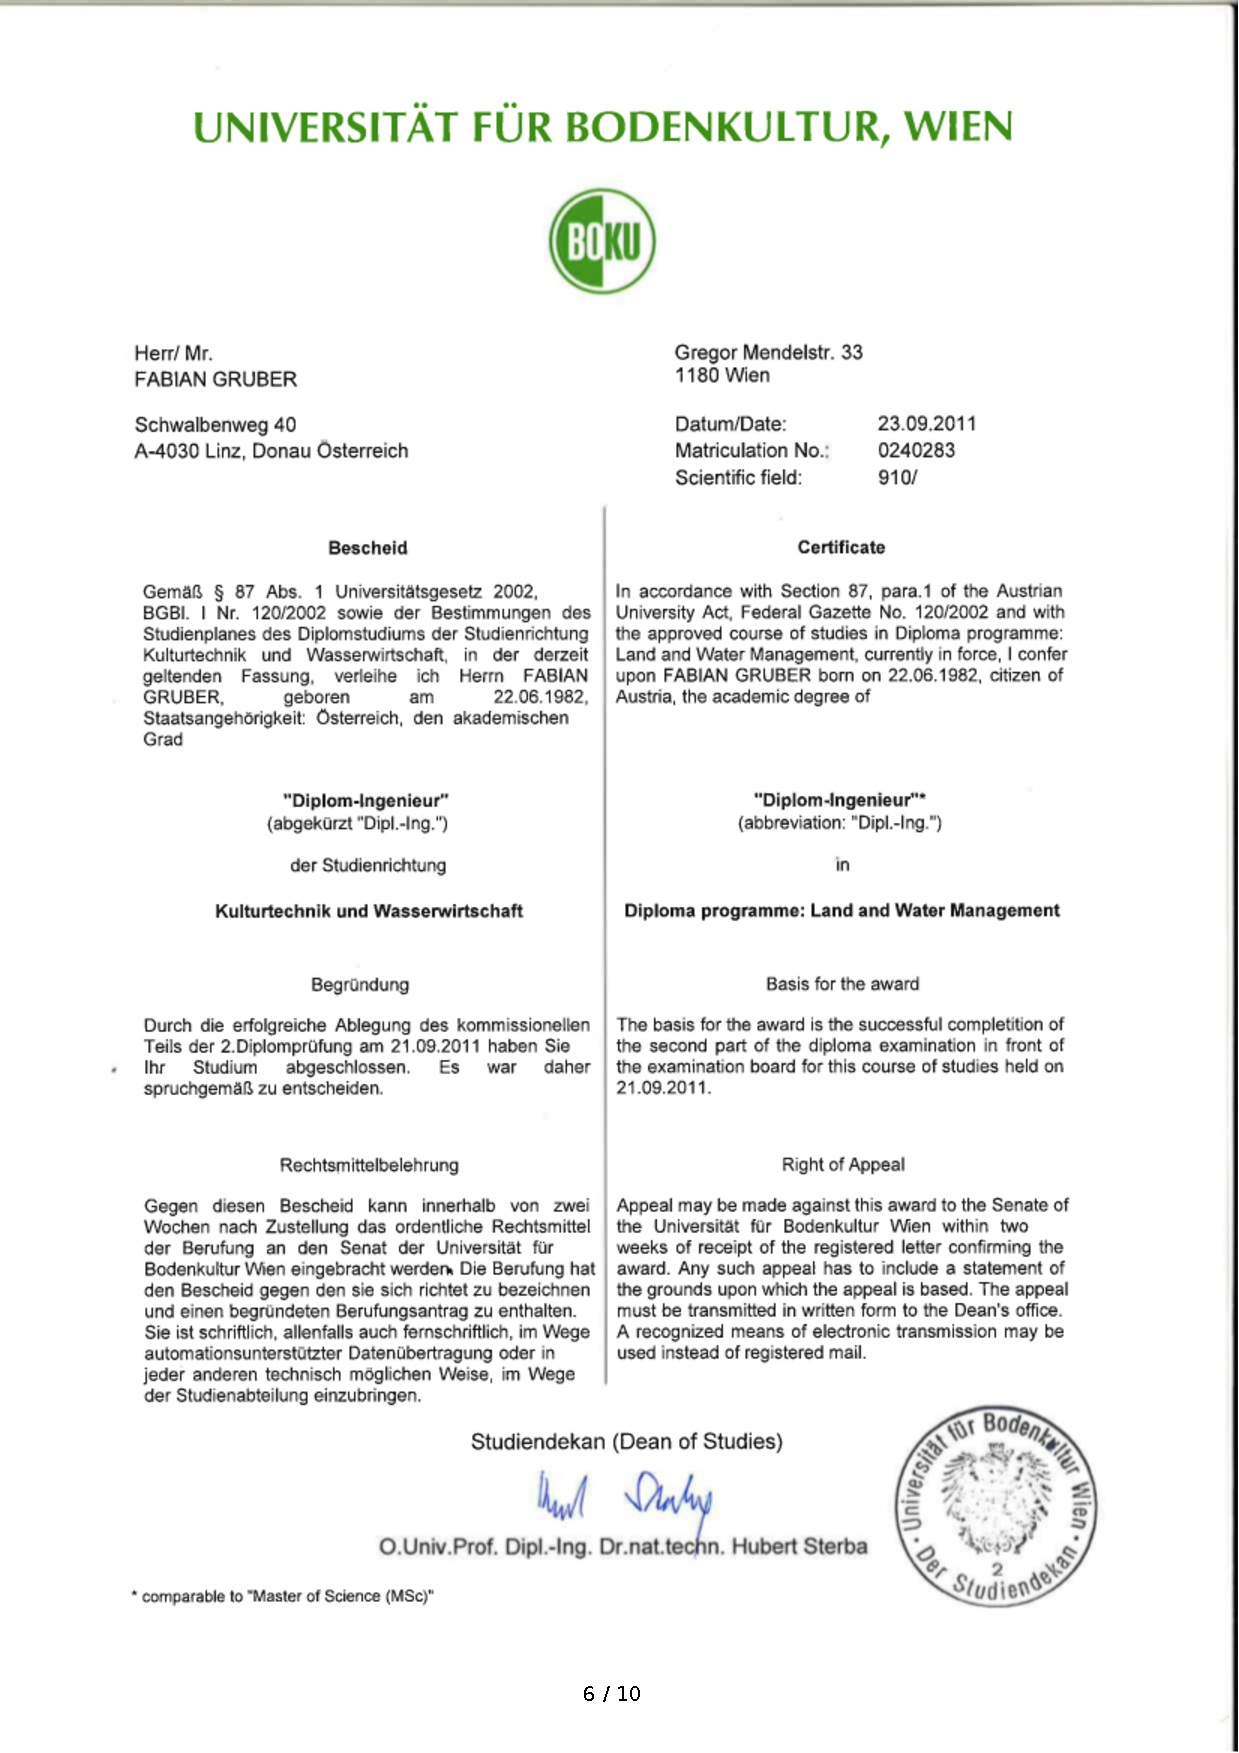
\includepdf{DP_6.pdf}
%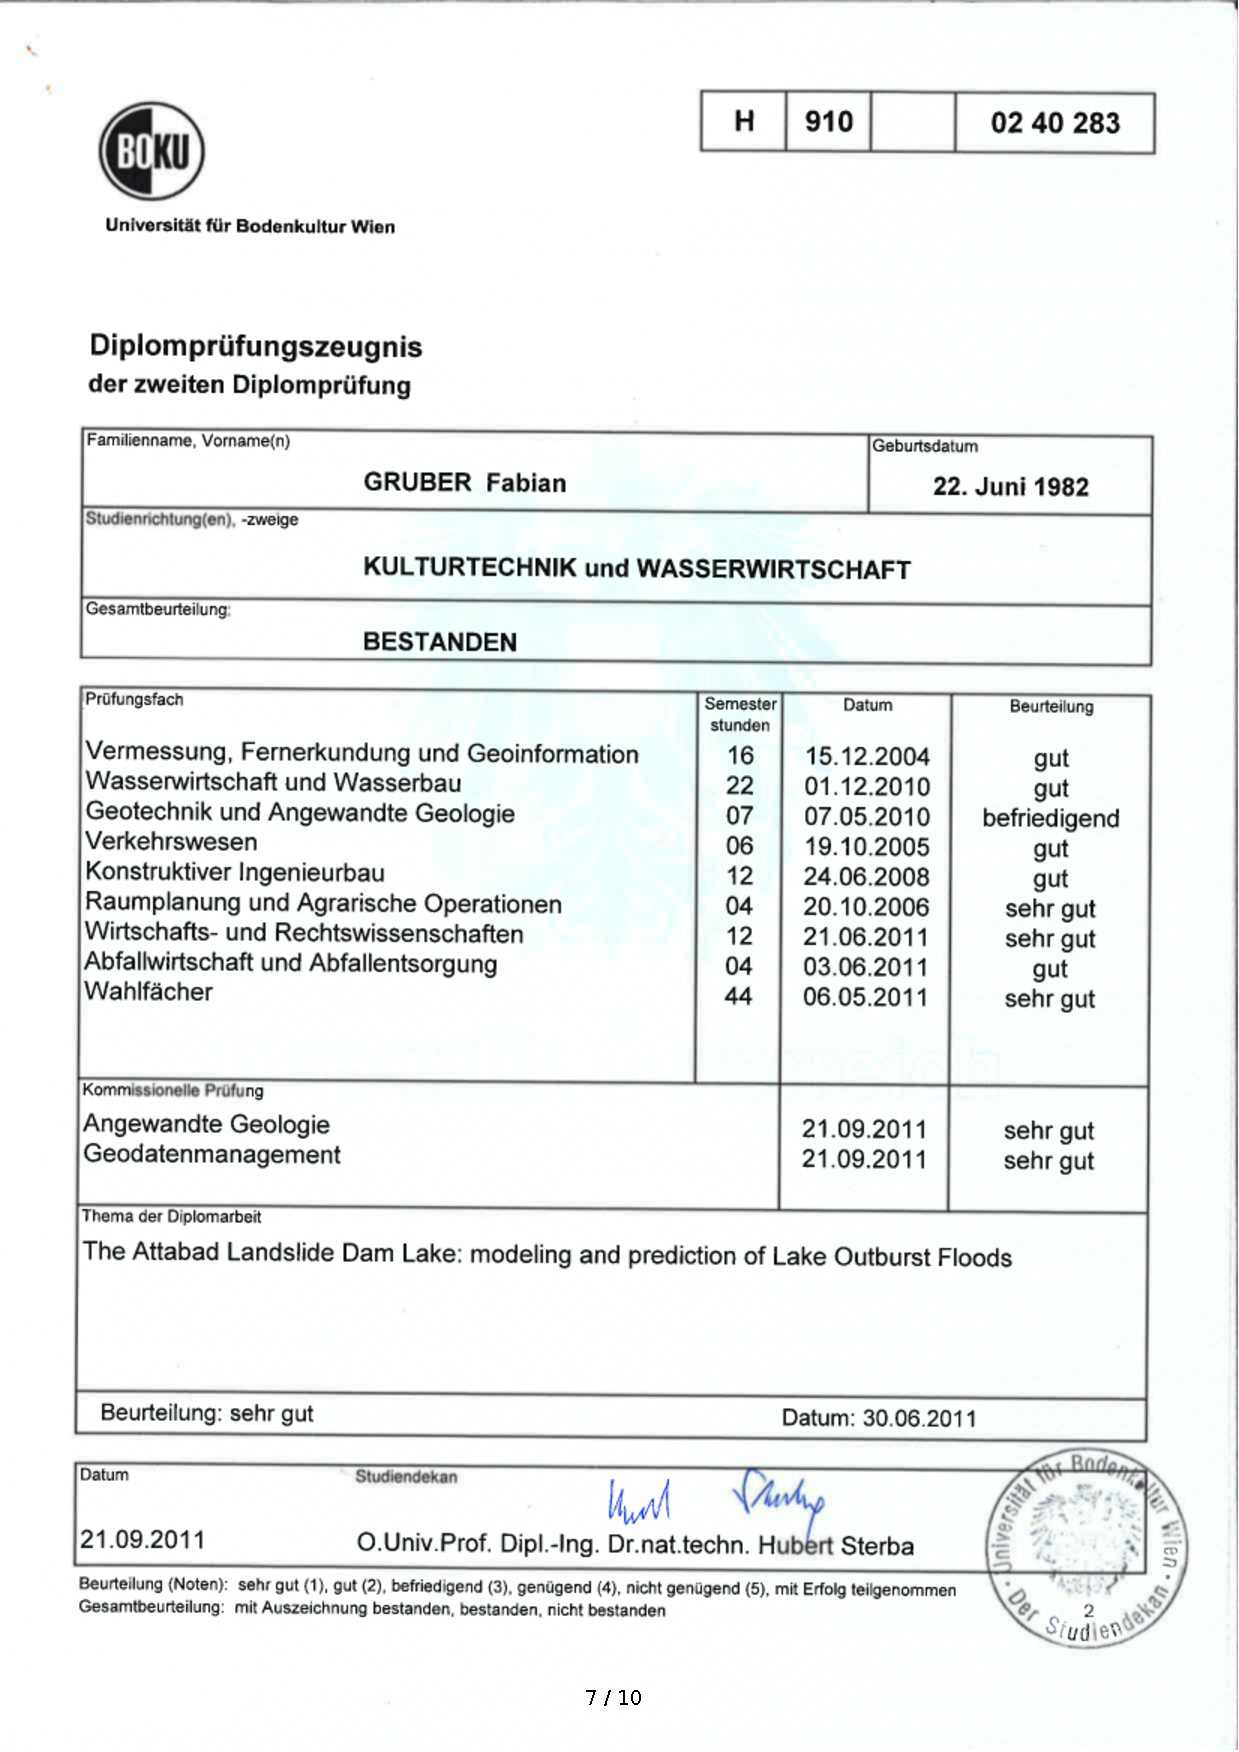
\includepdf{DP1_7.pdf}
%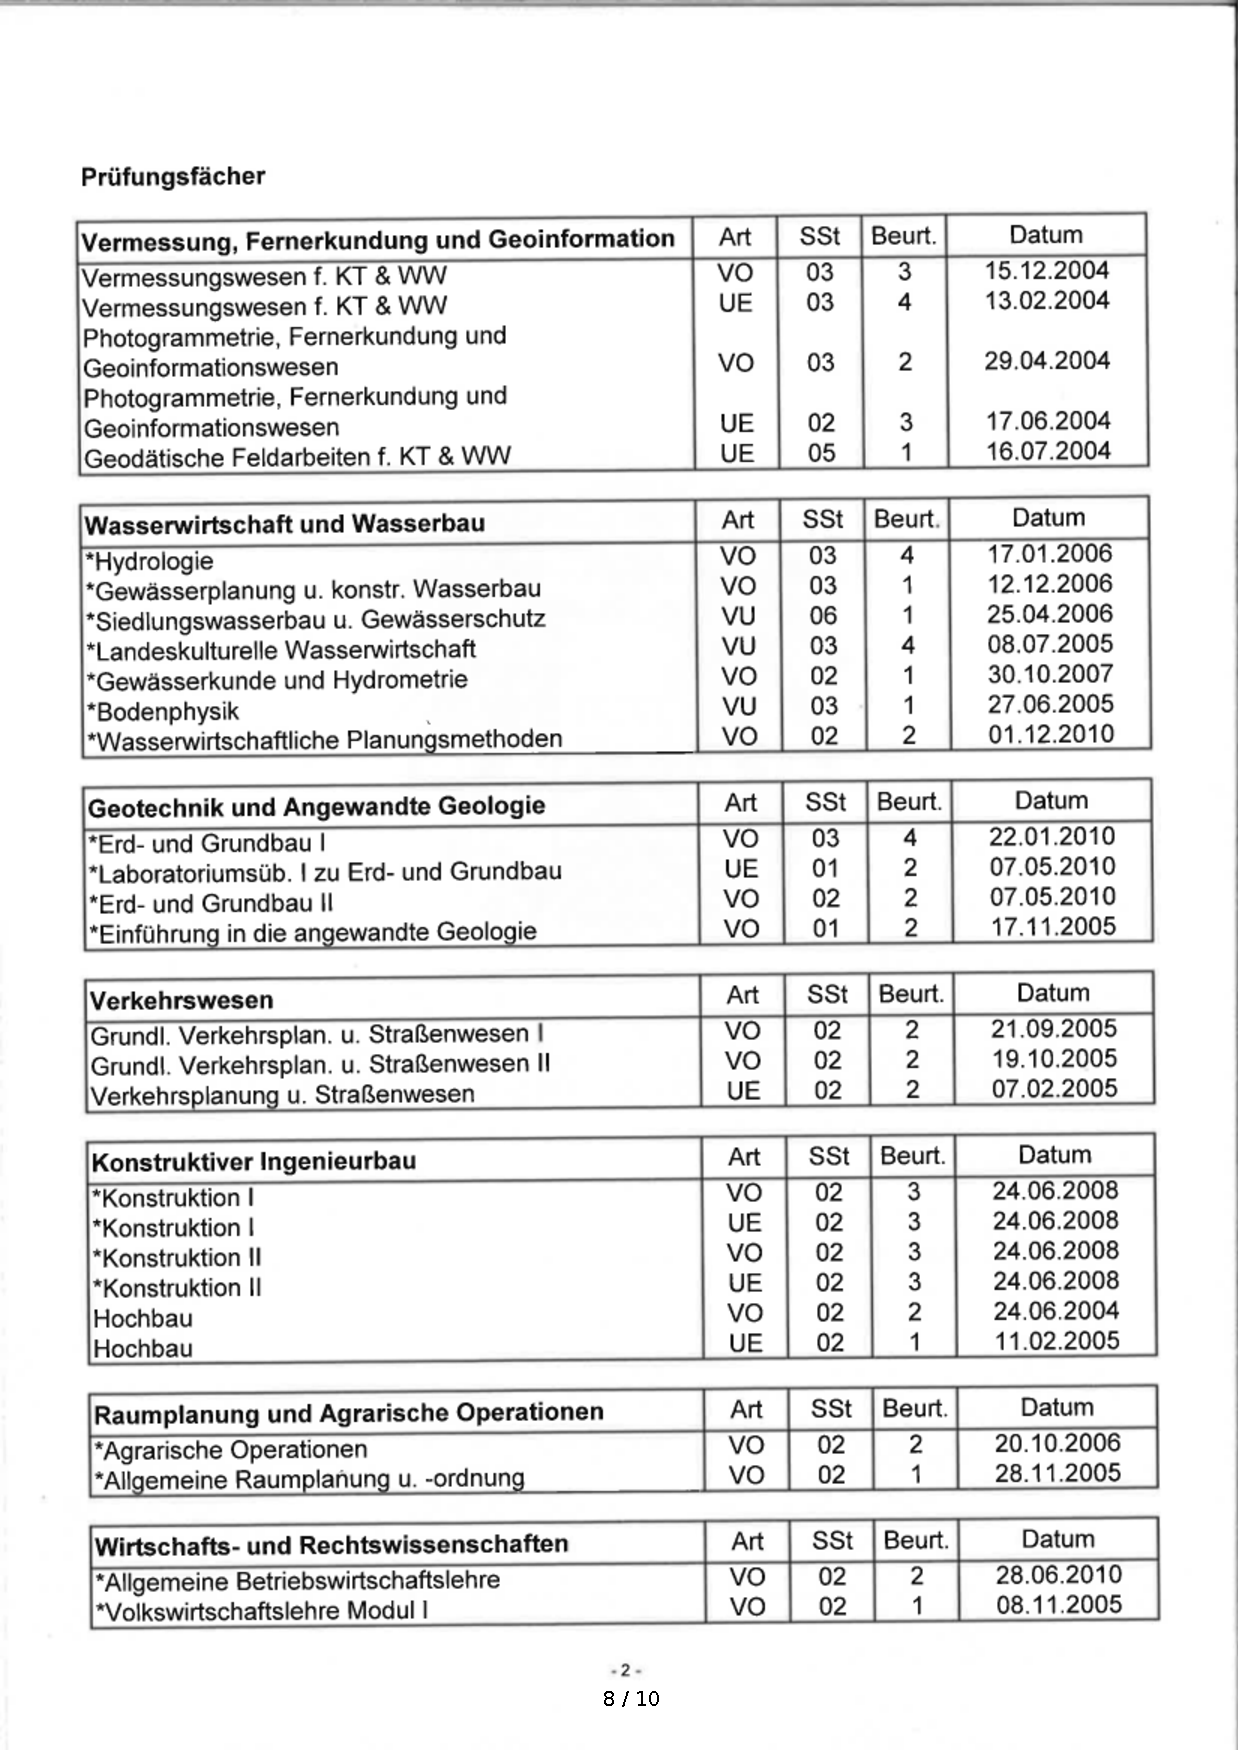
\includepdf{DP2_8.pdf}
%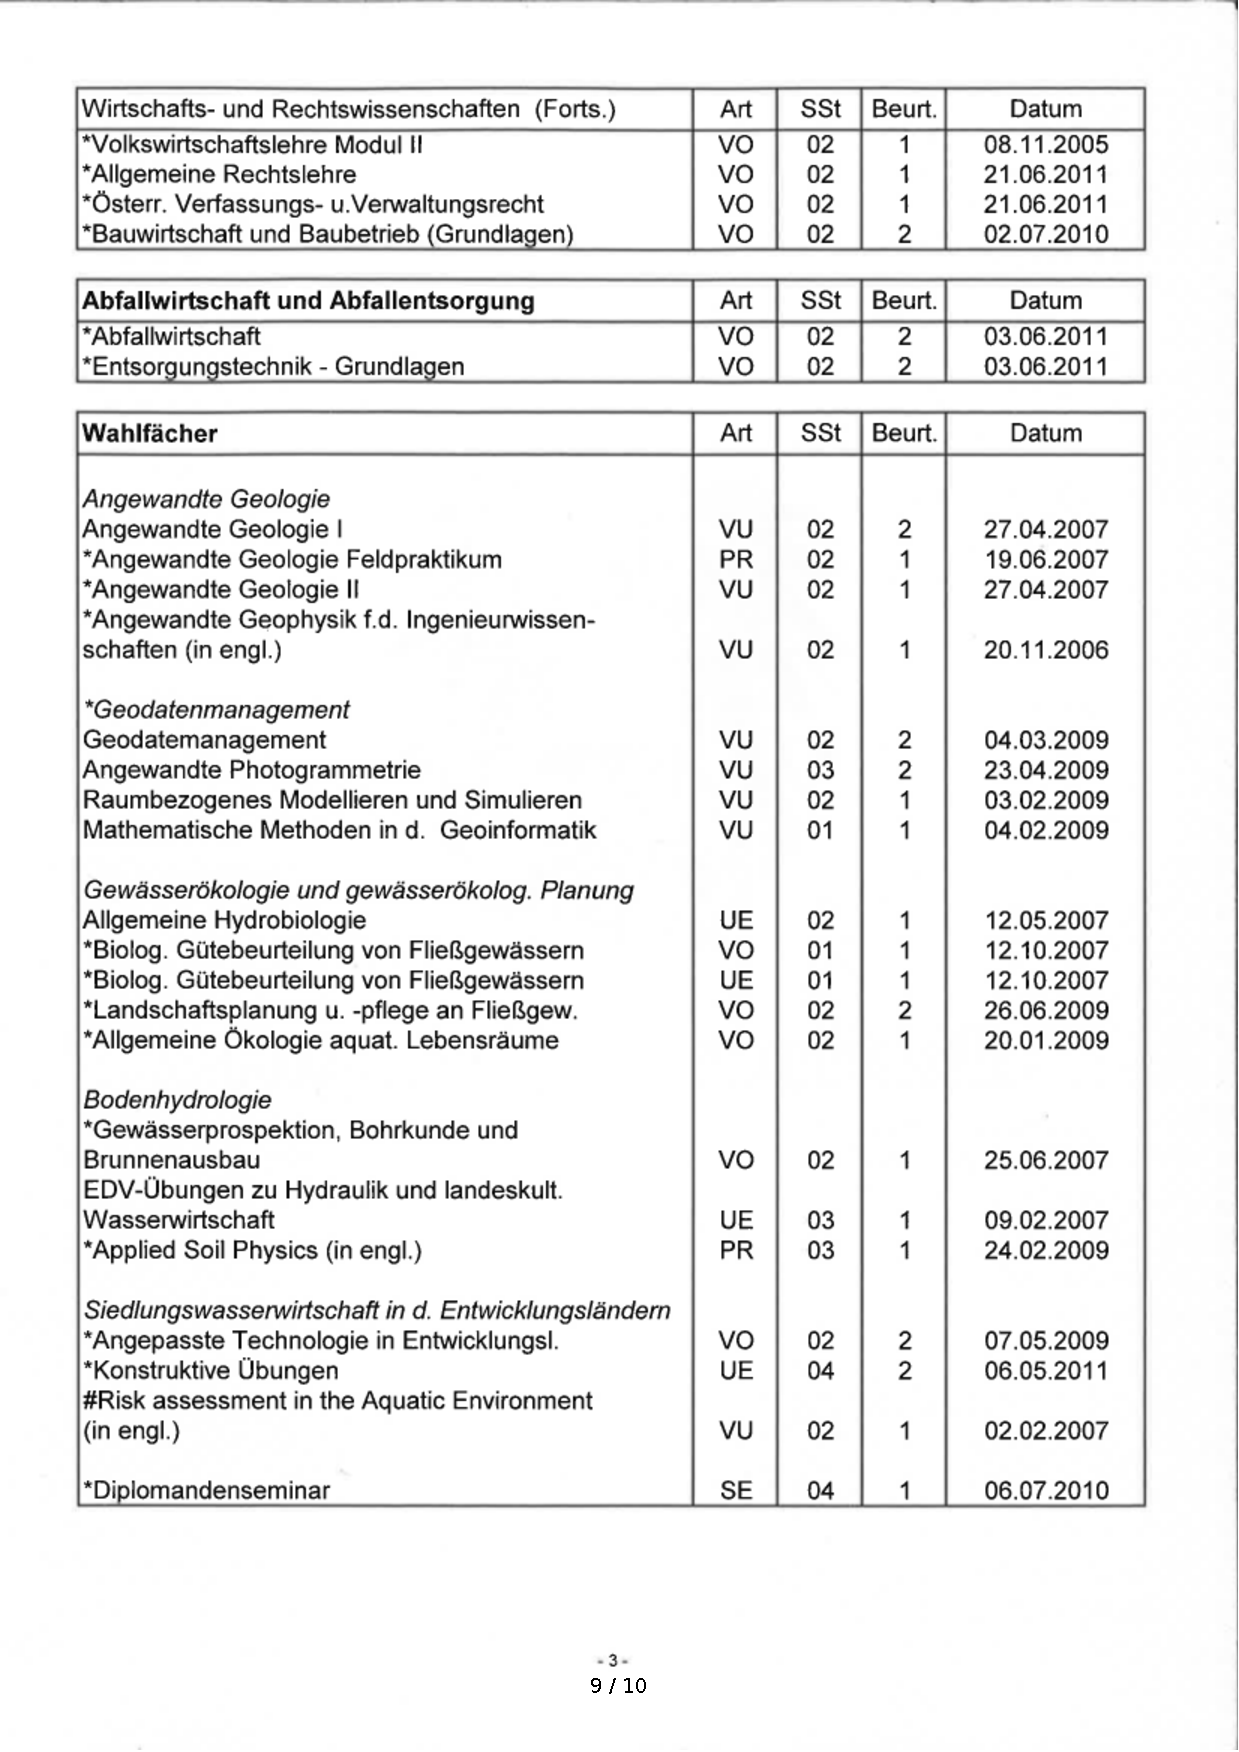
\includepdf{DP3_9.pdf}
%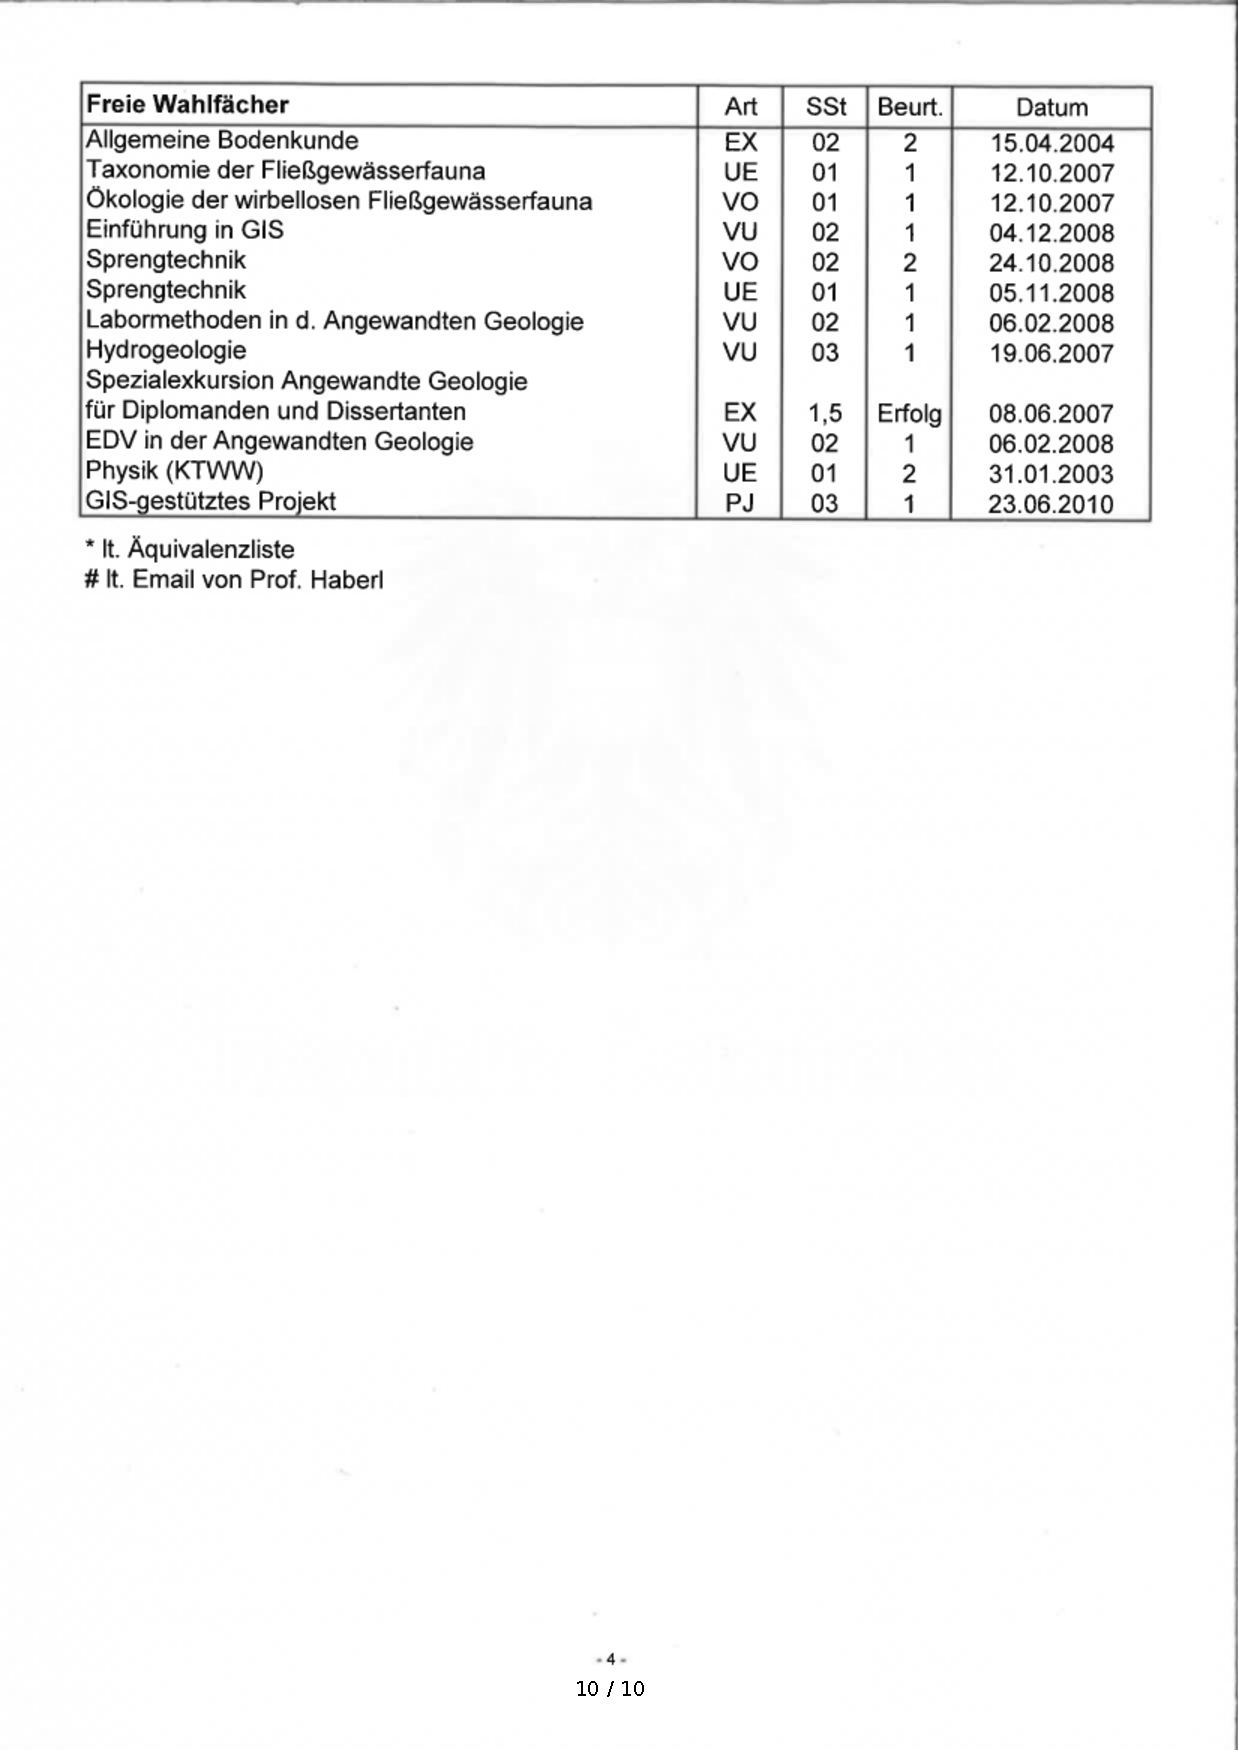
\includepdf{DP4_10.pdf}
\end{document}


%% end of file `template.tex'.
